\renewcommand{\SS}{\mathbb{S}}
\newcommand{\Par}[2]{\mbox{$( #1, #2 )$}}

\chapter{Uvod do studia struktury RNA}

Na zaciatku prace strucne zoznamime citatela s pojmamy, ktore s RNA a jej strukturou suvisia.

\section{Co je RNA}

Nositelkami genetickej informacie bunky su molekuly nukleovych kyselin
tvorene retazcami nukleotidov, ktore su zakladnymi stavebnymi jednotkami
nukleovych kyselin. Vyskytuje sa niekolko variant nukleotidov (baz). U RNA su to
adein (A), guanin (G), cytozin (C), uracyl (U),
pri DNA sa namiesto uracylu vyskytuje tymin (T).
Medzi jednotlivymi bazami sa mozu vyskytovat vodikove vazby. Nukleotidy maju
vzajomnu preferenciu, co znamena, ze bazy vznikaju najcastejsie medzi A-U a C-G
u RNA a podobne A-T a C-G u DNA.
Medzi jednotlivymi bazami existuju vazby na principe komplementarity.
Vodikove vazby existuju medzi bazami A-U a C-G u RNA a podobne A-T a C-G u DNA.
Strukturu nukleovych kyselin mozeme chapat podla stupna zjednodusenia
\begin{itemize}
	\item Primarna struktura - je urcena poradim jednotlivych nukleotidov
		do polynukleotidoveho retazca
	\item Sekundarna struktura - je dana parovanim medzi bazami molekuly
	\item Terciarna struktura - 3D priestorove usporiadanie molekuly
\end{itemize}
DNA je dvojvlaknova molekula u ktorej spojenie medzi vlaknami sa realizuje na principe
komplementarity.
Naopak, RNA je iba jednovlaknova molekula a v snahe minimalizovat volnu energiu molekuly
sa paruje sama na seba. V tomto hraju rolu pritazlive sily medzi bazami.

V praci budeme strukturou mysliet prave sekundarnu strukturu RNA, ak nebude povedane inak.

Az donedavna sa myslelo, ze funkcia RNA je obmedzena na prenos genetickej informacie z DNA
v jadre bunky do ribozomu. Napriklad pri tvorbe bielkovin (mRNA), alebo transporter aminokyselin
v ribozome bunky (tRNA).
% TODO: citacie k druhom RNA
Avsak existuje mnoho dalsich, od relativne
malych molekul tvorenych desiatkami baz, ktore pomahaju pri expresii genov
(miRNA, siRNA, tmRNA a dalsie), az po velke, tvorene tisickami nukleotidov (rRNA).

\section{Sekundarna struktura rRNA + konzervovanost}

Ako hlavny objekt zaujmu sme si spomedzi vsetkych druhov RNA vybrali prave ribozomalnu,
najma kvoli jej velkosti a tomu, ze existujucim nastrojom prave velkost robi najvacsie problemy
pri vizualizacii.

\begin{definice}[Primarna struktura RNA]
  \label{def:RNA_primarna_struktura}
	Nech $\Sigma$ je abeceda $\{A, C, G, U\}$. Potom slovo $W \in \Sigma^n$ nad touto abecedou
	je sekvencia nukleotidov (baz) RNA.
\end{definice}

Jednotlive nukleotidy sekvencie RNA budeme, ak bude jasne o co ide, oznacovat priamo poradovym
cislom, teda $i$ bude oznacovat nukleotid $W_{i}$, resp. $W[i]$.

\begin{definice}[Sekundarna struktura RNA]
  \label{def:RNA_sekundarna_struktura}
	Nech $W$ je sekvencia podla definicie \ref{def:RNA_primarna_struktura} dlzky n.
	Sekundarnou strukturou oznacime mnozinu $\SS$ parov nukleotidov \Par{i}{j} takych, ze
	pre dva pary \Par{i}{j} a \Par{k}{l} $\in \SS$ (bez ujmy na obecnosti $i \leq k$)
  plati jedno z nasledujucich:
	\begin{itemize}
		\item $i = k \iff j = l$
		\item $i < j < k < l$, cize par \Par{i}{j} predchadza par \Par{k}{l}
		\item $i < k < l < j$, cize par \Par{i}{j} obsahuje par \Par{k}{l}
	\end{itemize}
\end{definice}

%TODO: obrazok prim/sek/terc struktury RNA

Prva podmienka zabezpecuje, ze nukleotid je najviac v jednom bazickom pare, druha a tretia
hovoria o usporiadani parov, bud su na sebe nezavisle alebo na seba nadvazuju.
Posledna podmienka zakazuje existenciu pseudouzlov (pseudoknots).

%TODO: pseudoknot obrazok
%TODO: 2 obrazky RNA napriec fylogenetickym stromom

\begin{figure}[H]
\centering
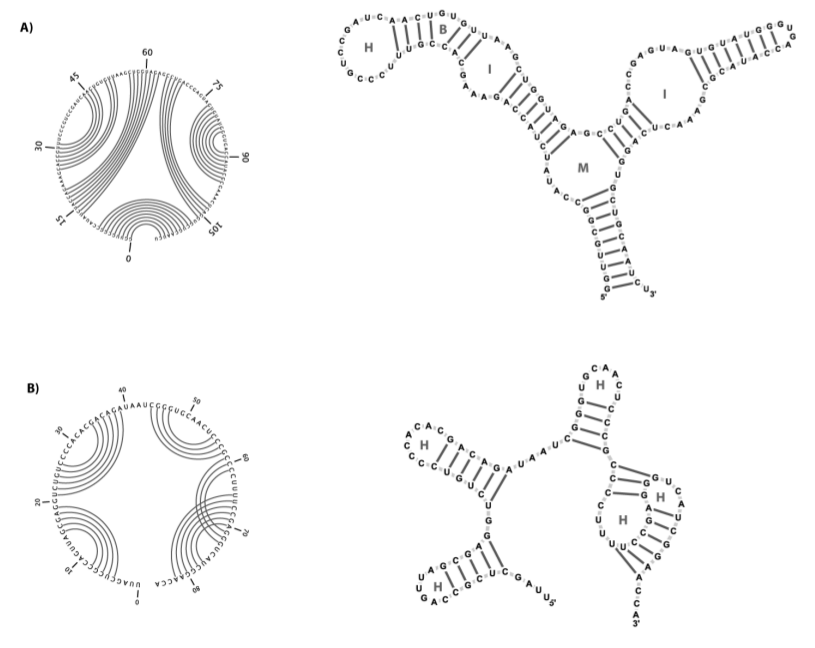
\includegraphics[width=140mm, height=120mm]{../img/RNA_circular_reprezentation.png}
\caption{Circular Feynman - kruhova reprezentacia sekundarnej struktury}
\label{obr:RNA_circular_representation}
\end{figure}


\subsection{Motivy}

Motivom v RNA mame na mysli casti molekuly, ktore vytvaraju urcite struktury.
Na obrazku \ref{obr:RNA_motifs} vidime motivy, ktore sa mozu v RNA vyskytovat.

Stem (stonka) je cast molekuly kde sa na seba paruju dva suvisle casti RNA vlakna.
Interior loop spaja dva stemy a medzi nimi na oboch stranach obsahuje nesparovane
bazy. Podobna je bulge (vypuklina), ale nesparovane nukleotidy ma iba z jednej strany.
Hairpin je medzi castami vlakna ktore sa paruju sami na seba.
Multibranch loop je podobna ako interior loop, ale spaja dokopy viac stemov.
V dalsom rozpravani nam bude stacit rozdelenie na stem a loop.

%TODO: ako nazyvat strukturne motivy v RNA: anglicky, alebo hladat vhodny preklad

\begin{figure}[H]
\centering
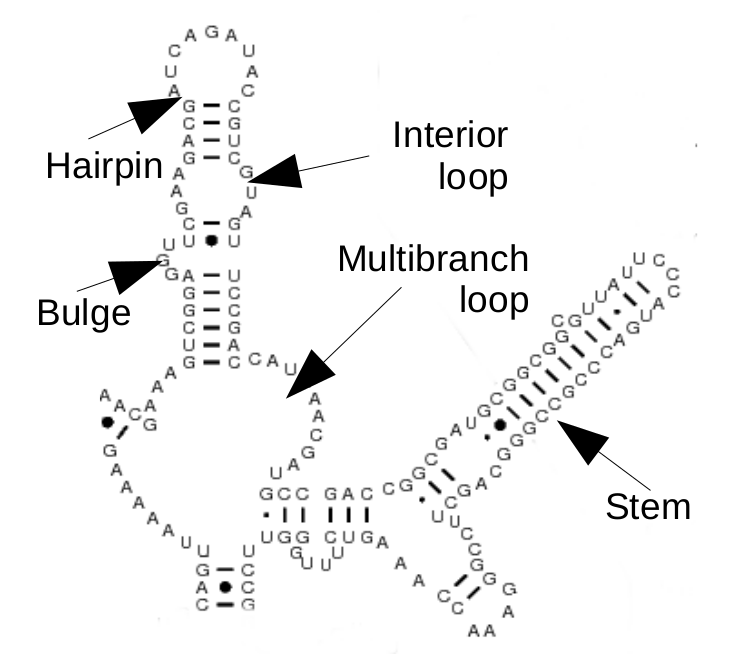
\includegraphics[width=70mm, height=70mm]{../img/struktury_v_rna.png}
\caption{Strukturalne motivy v RNA}
\label{obr:RNA_motifs}
\end{figure}

